\subsection{Main features}
\begin{figure}[!h]
    \centering
    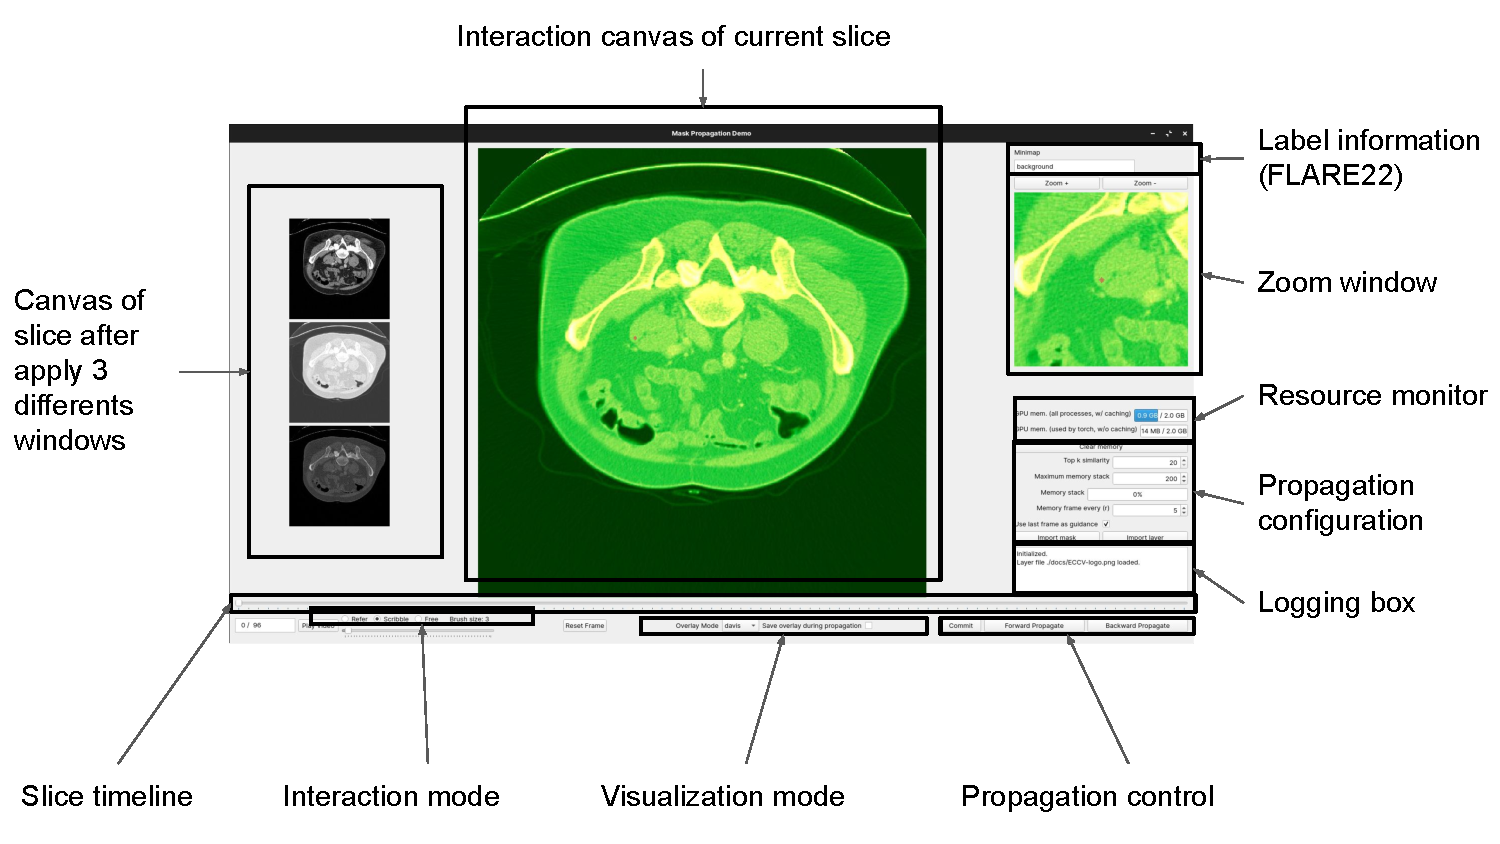
\includegraphics[width=\textwidth]{content/resources/new_images/application/GUI.pdf}
    \caption{The layout of our annotation tool}
    \label{fig:gui_app}
\end{figure}

% \textbf{Preview and select annotated slices}: 
% By using \textbf{slice timeline}, annotator can choose a arbitrary slice by dragging the slider. In each timestamp, two main canvas will be previewed corresponding: On the left side is the visualization of applied image on different window as we demonstrated before on section \ref{sec:preprocess}; The large main one is displays the concatenate image from 3 preprocessed image as a RGB image. The canvas on the right hand is the zooming window, increase the crop image size for small details interaction. The zoom in ratio could be modify by nearby zooming controller buttons, or maybe scroll wheel to zoom in and out.

% \textbf{The main controls include}: Using left and right mouse buttons for positive and negative clicks, or scribbles modify an existing mask respectively, press space to finish the current object; pressing the left arrow key displays the previous image, and pressing the right arrow key displays the next image, pause when correction is needed. Using the \textbf{propagation control} to propagate through the whole volume. The target object must be selected by using the number keys. "1" corresponds to the first object, etc. 

% \textbf{The monitors}: Stats would be printed on the logging box. The resource monitor also displays the GPU memory exists. Label information would be on the top right shows the information of hovering object.

% \textbf{The interactions}: We provide 3 type of interactions including: scribbles to mask, free scribbles and reference. 

\textbf{Selecting and previewing the annotated slices}: 
By using the \textbf{slice timeline}, the annotator can choose any arbitrary slice just by dragging the slider. In each timestamp, two main canvas are shown: on the left side is the visualization of applied image on different windows due to the aforementioned pre-processing stage (as in \ref{sec:preprocess}); The larger canvas in the middle displays the stacked version of the 3 images as a RGB image. 
We also provide the user with an additional canvas on the left side, which illustrates the zooming view of the main canvas for small details interaction. The zoom-in ratio could be modified by available controller buttons, or by scrolling the mouse wheel.Users can also navigate through the timeline by pressing the left arrow key and the right arrow key. 

\textbf{Performing slice annotation}: 
We provide 3 type of annotation interactions including: scribbles to mask (s2m), free scribbles and automatic reference. In the free scribble mode, the user can freely draw on the canvas to create object masks. Meanwhile, The s2m and reference options offer the ability to use deep learning models to automatically generate the masks. 
% Options are demonstrated in the \textbf{interaction mode}. 
The list of available objects can be shown by pressing "L". Then to choose a specific object that the user desire to label, corresponding keypad should be pressed. For example, to annotate an object that belongs to class "1", keypad "1" should be pressed. In both the scribbles modes, the user can use left and right mouse buttons to draw new masks or to erase existing masks respectively. After finishing, the user can press space to obtain the mask. With the initial mask formed, the user can perform forward/backward propagation to disseminate the annotated mask to other slices across the timeline. The \textbf{propagation control} provides options to accomplish that.

\textbf{The monitors}: Stats are printed in the \textbf{logging box}. The \textbf{resource monitor} also displays the current usage of GPU memory. Label information is also shown on the top right, indicating the information of the  object that is being hovered on.